\chapter{Project description}
\pagenumbering{arabic}
%\addcontentsline{toc}{chapter}{Project description}
The system is composed by:
\begin{enumerate}
\item A DC direct drive brushed motor
\item Three carts
\item Three springs
\item Several weights
\item Three encoders for the position
\item A PoliArd board
\end{enumerate}
The mechanism consists of up to three mass carriages interconnected by bi-directional springs. The mass carriage suspension is an anti-friction ball bearing type with approximately $\pm 3$ \SI{}{\cm} of available travel. The linear drive is comprised of a gear rack suspended on an anti-friction carriage and pinion coupled to the motor shaft. Optical encoders measure the mass carriage positions.\\

Three springs can be attached between the carts or between the first cart and the base plate and the mass of all the carts can be adjusted using the weights provided ($500 \pm 5$ g each).\\

The encoder type is CP-850-4000-ECP: it is an optical incremental digital rotary shaft encoder. The number 4000 indicates the line counter (i.e. the number of equally spaced radial lines per 360 mechanical degrees on the incremental encoder code disk). Moreover has a resolution of $14$ bits.\\A low power light source is used to generate two 90 degrees out of phase sinusoidal signals on the detectors as the moving plate rotates with respect to the stationary plate. The moving plate rotates by means of an iron string wound up in it and then attached to the cart. The position is measured by calculating the angular displacement of the disk.The motor encoder is used to transmit both voltage and current to the Arduino board. \\

The 24 Volt DC motor has a case diameter of 63 mm and 194 Watts of output power. It has a nominal speed of 3700 rpm and a nominal Torque of 270 \SI{}{\milli\newton \meter}. The DC motor has nominally a resistance of 2 $\cdot$ 0.7 \SI{}{\ohm} and an inductance of $2\cdot$ 1.05 \SI{}{\milli \henry}.\\

The poliArd board mounts an Arduino Due board. The board has a 24 \SI{}{\volt} power supply and it’s capable of measuring up to 5 \SI{}{\ampere} current. It has two motor drivers and four encoder interfaces. The board is programmable and the control strategy can be implemented using Matlab 2015a. To power on the board the user has to flip the first lever from the left. The other two levers can be programmed freely.
\subsection{Sampling frequency}
During the course of the project the chosen sampling frequency was $f_s = 200 Hz$.  This allowed us not to worry about issues such as: the additional phase due to sampling, identification, etc...
\section{Issues}
\subsection{Motor saturation}
From simple test it’s easy to see that measured current saturates. What can be observed is that even though the current reaches a maximum value, the cart continues to move so this means that the sensor is not able to measure above a given current. In particular, it can be seen from Figure \ref{fig:sensorsaturation} that the sensor saturates to $4.42$ \SI{}{\ampere} and to $-10$ \SI{}{\ampere}.\\
In any case the Arduino Due cannot reliably measure more than 5 \SI{}{\ampere} current as the data-sheet specifies, so from this point onward we will limit all test currents to 5 \SI{}{\ampere} in both directions. Even in this way a difference remains between positive and negative measured current.  
  \begin{figure}[!h]
  	\centering
  	\subfloat[Negative maximum current]{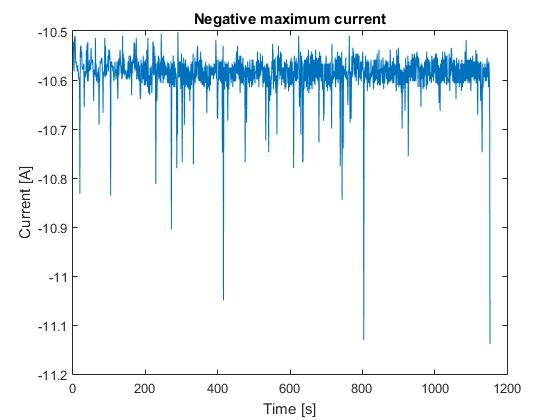
\includegraphics[width=0.3\textwidth]{img/neg_max_current.jpg}}
  	\subfloat[Positive maximum current]{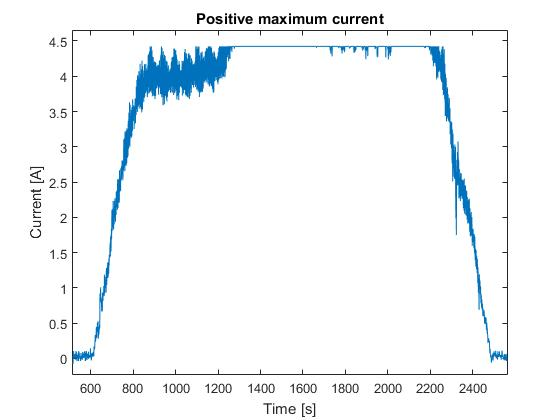
\includegraphics[width=0.3\textwidth]{img/pos_max_current.jpg}}
  	\caption{Sensor saturation effect}
  	\label{fig:sensorsaturation}
  \end{figure}
\subsection{Current noise}
After applying the protector to the system we measured the current noise at different current levels.\\ \\
First of all we noticed that the current has a Gaussian distribution, with some deterministic components. This was done by using a step signal equal to $1$ as input voltage to the motor and taking an histogram of the current at steady state and its Fast Fourier Transform (after detrending). This is seen in figure \ref{fig:currnoise1}. 
  \begin{figure}[!h]
  	\centering
  	\subfloat[Current at steady state]{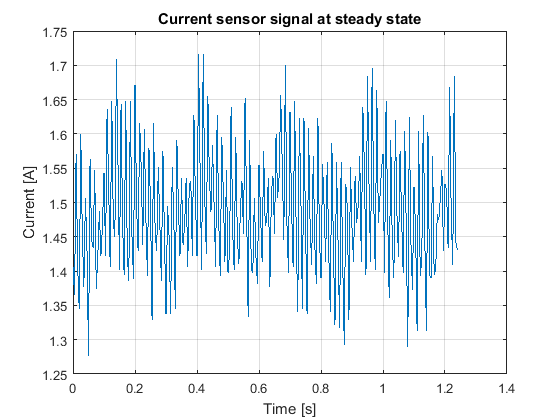
\includegraphics[width=0.3\textwidth]{img/cur1.png}}
  	\subfloat[Histogram of the current]{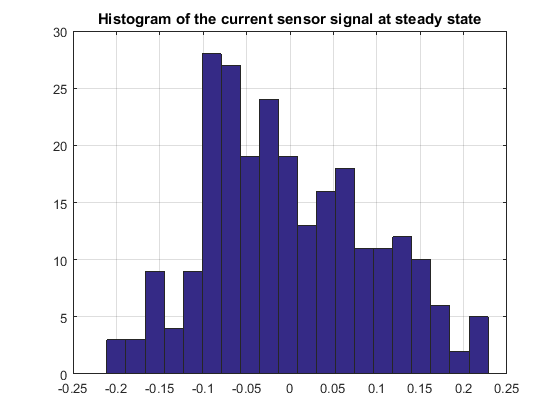
\includegraphics[width=0.3\textwidth]{img/cur2.png}}
  	\subfloat[FFT Plot]{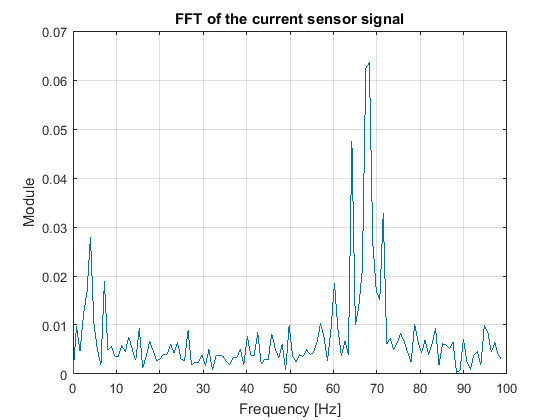
\includegraphics[width=0.3\textwidth]{img/cur3.png}}
  	\caption{On the left: the current sensor signal at steady state. On the center its histogram plot after detrending. On the right its FFT after detrending.}
  	\label{fig:currnoise1}
  \end{figure}
This is an important step, since a current control loop was necessary for $2$ and $3$ degree of freedom. Therefore we needed a filtered output of the current signal. And we needed to understand how to filter the output of the sensor.
 \\Later we applied a ladder type signal to measure the noise when the current was constant at different current levels. In fact we noticed that the noise variance increased for increasing values of $v$. From the measurements obtained it can be seen that the variance of the negative current increases as the current increases in modulus instead if the current is positive the variance is small and almost constant. The fault of this behaviour for negative current is probably of the current measurement system.\\
\def\arraystretch{1.2}
\begin{table}[]
\centering
\caption{Variance and mean of the current sensor for different voltage inputs.}
\label{my-label}
\begin{tabular}{lllll}
\cline{1-2} \cline{4-5}
\multicolumn{1}{|l|}{$\mathbb{E}[i(t)], v < 0$} & \multicolumn{1}{l|}{var$(i(t))$, $v<0$} & \multicolumn{1}{l|}{} & \multicolumn{1}{l|}{$\mathbb{E}[i(t)], v >0$} & \multicolumn{1}{l|}{var$(i(t))$, $v>0$} \\ \cline{1-2} \cline{4-5} 
-0.020                                          & 0.0015                                  &                       & -0.022                                        & 0.0014                                  \\
-0.554                                          & 0.0035                                  &                       & 0.683                                         & 0.0013                                  \\
-1.758                                          & 0.0119                                  &                       & 1.568                                         & 0.0015                                  \\
-2.703                                          & 0.0274                                  &                       & 2.312                                         & 0.0016                                  \\
-3.964                                          & 0.0359                                  &                       & 3.182                                         & 0.0016                                  \\
-5.454                                          & 0.0523                                  &                       & 4.316                                         & 0.0022                                  \\ \cline{1-2} \cline{4-5} 
\end{tabular}
\end{table}

From the variance values of the current for $v(t)<0$ it can be seen that the variance grows linearly with the modulus of the current, whilst for $v(t)>0$ is almost constant, with average value $0.0016$. Therefore for $v(t)<0$ we decided to estimate the variance by simple linear interpolation:
\begin{equation}
\text{var}(i(t)) = a + b \mathbb{E}[i(t)]
\end{equation}
by means of least squares interpolation:
\begin{equation}
\theta = (X^T X)^{-1} X^T Y, \quad
Y  = \begin{bmatrix} \text{var}(i_1)\\ \vdots \\ \text{var}(i_n) \end{bmatrix},
X = \begin{bmatrix} 1 & \mathbb{E}[i_1]\\ \vdots \\ 1 & \mathbb{E}[i_n] \end{bmatrix},
\theta = \begin{bmatrix} a\\ b\end{bmatrix}
\end{equation}
where $i_j$ represents the $j$-eth segment of current data taken from the ladder experiment. The result can be seen below.\\

All these experiment were done in order to estimate the variance of the current sensor and to have enough information to build the variance matrixes for the Kalman filter.
  \begin{figure}[!h]
  	\centering
  	\subfloat[]{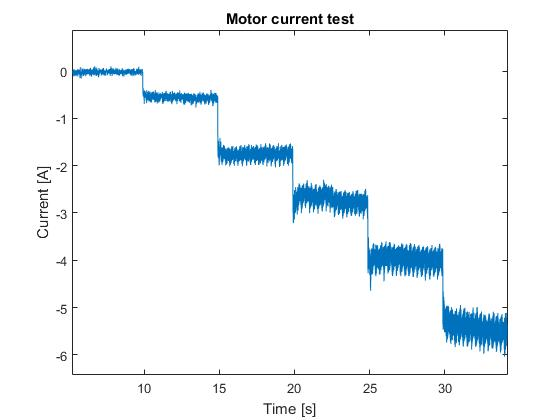
\includegraphics[width=0.3\textwidth]{img/neg_ladder.jpg}}
  	\subfloat[ ]{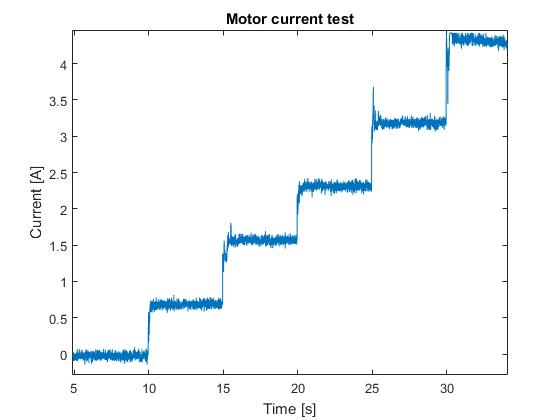
\includegraphics[width=0.3\textwidth]{img/pos_ladder.jpg}}
  	\subfloat[ ]{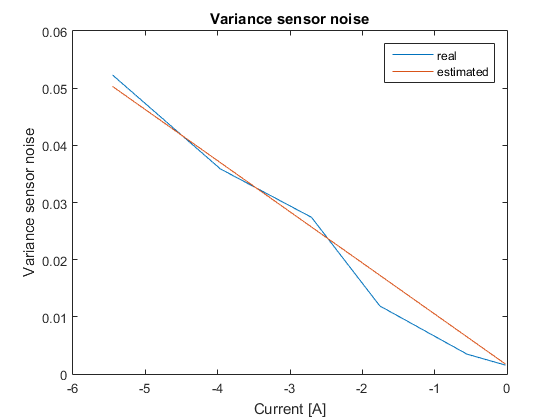
\includegraphics[width=0.3\textwidth]{img/current_variance_estimated.png}}
  	\caption{Ladder signal used for variance identification, and estimation of the current noise variance for $v<0$.}
 
  \end{figure}

\subsection{Encoder signal}
Another problem is the one of the signal given by the encoders. This signal is a voltage impulse given to the Arduino. Unfortunately, the measure showed by Poliscope is not in centimetres so a conversion was in order. The idea was to give a reference signal in an open loop configuration. Once the transient is passed both Poliscope value and the real displacement of the cart were measured. The average value  of the conversion gain is $559$ (steps to cm), with standard deviation $20$ (steps-to-cm). Tables with data are not shown in this report, but can be found at the GitHub directory of the project.
\section{System protection}
To avoid undesired behaviour of the system, a Simulink protection of the system has been designed. The system monitors current, voltage and displacement and if they overshoot a given value an alert is triggered that switches off the system to prevent any damage. 
Moreover, Arduino Due doesn’t behave very well when the reference signal starts at the same time of its power on. For this reason, the system has been designed in order to start the signal only after 3 seconds the user pushed the lever number 2. This logic has been implemented using a finite state machine through the library Stateflow in Matlab.
The system is composed by four macroblocks: Input Manager, Protector, System, Controller.
\begin{figure}[h]
	\centering
	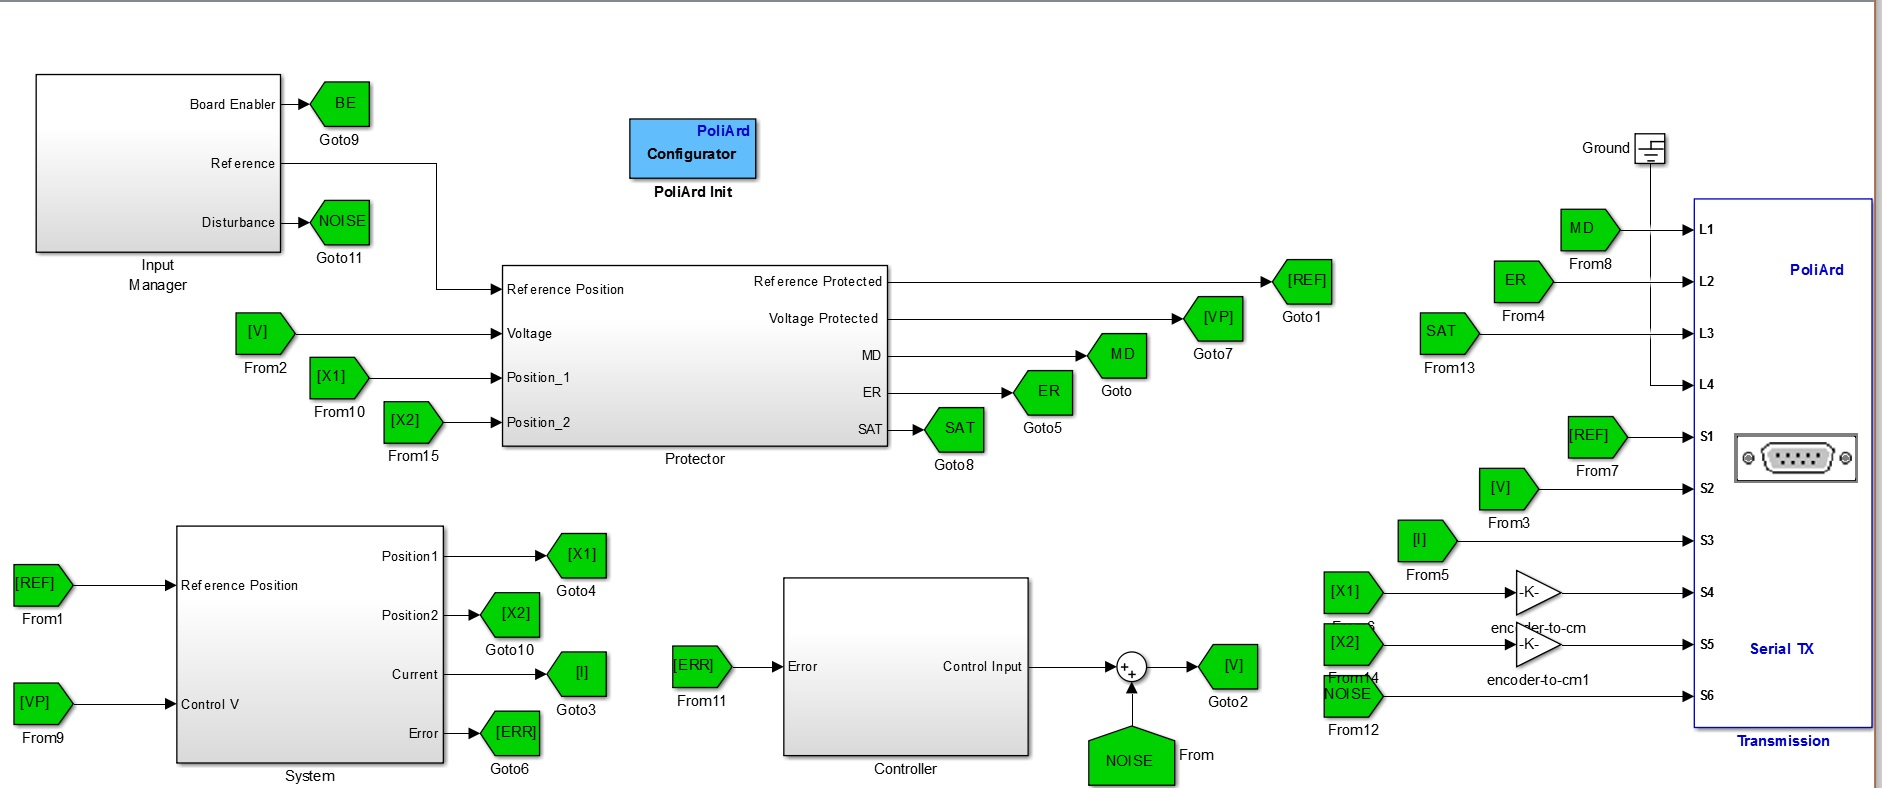
\includegraphics[width=0.8\textwidth]{img/overall_condom.jpg}
	\caption{Overall protection scheme}
\end{figure}

\subsection{Input Manager}
With a manual switch we can choose between potentiometers and reference signals. With the two levers we can decides instead the function of those potentiometers. 
If the second switch of the Arduino board is enabled then one potentiometer is a disturb for the control input instead the other one is used as variable reference signal. 
If the third switch of the Arduino board is enabled then both the potentiometers are used as reference but one is positive and one is negative. 
 \begin{figure}[!h]
 	\centering
 	\subfloat[Startup state machine]{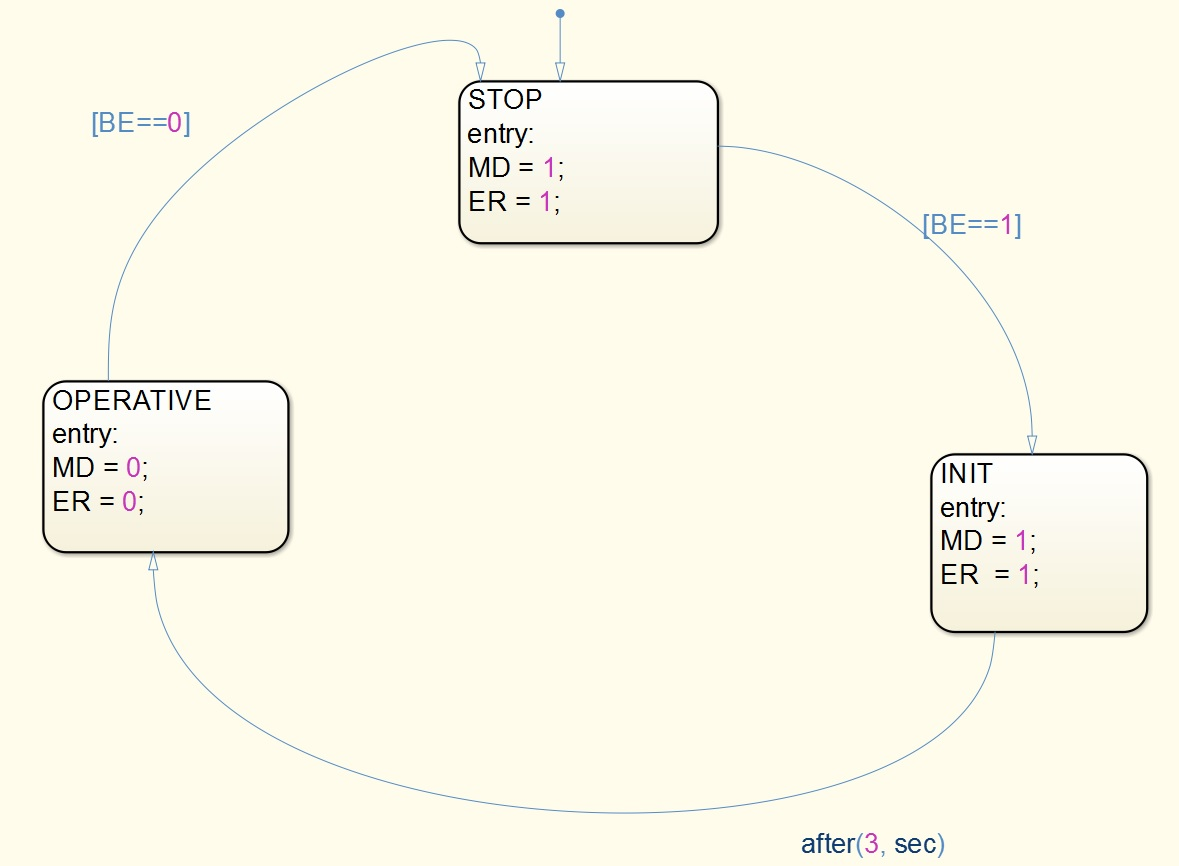
\includegraphics[width=0.3\textwidth]{img/init_manager.jpg}}
 	\hspace{1cm}
 	\subfloat[Alert state machine]{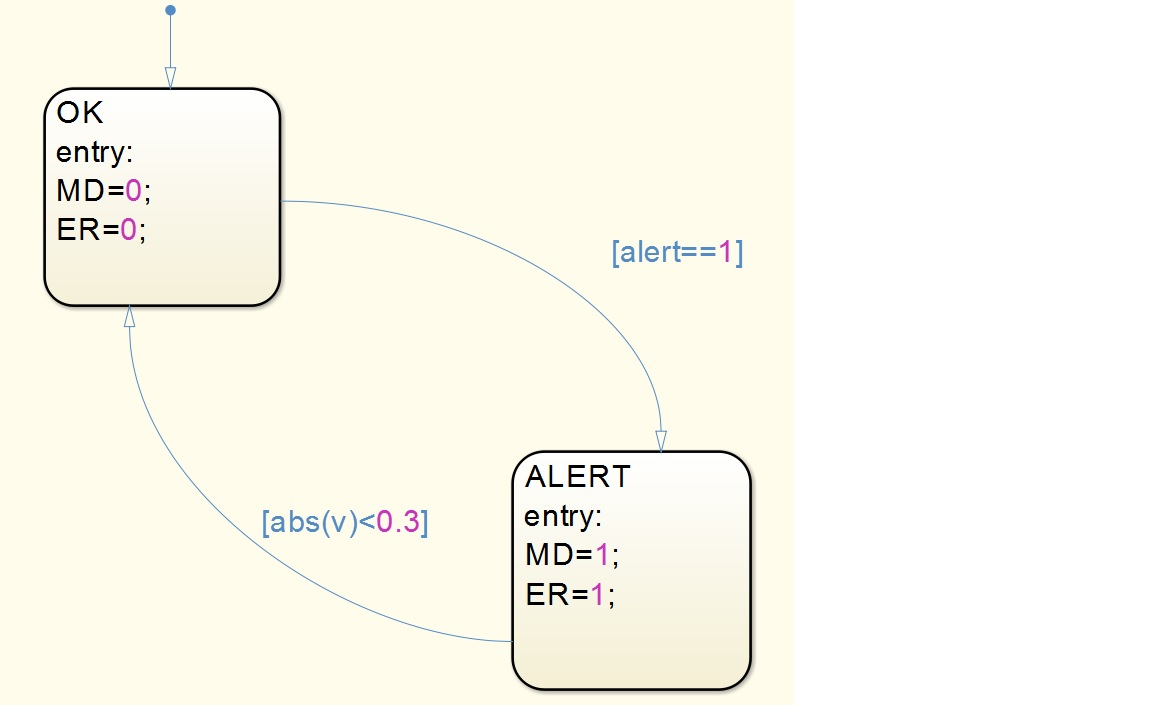
\includegraphics[width=0.33\textwidth]{img/alert_manager.jpg}}
 	
 	\caption{State machines used for startup of the system and alert signaling.}
 	
 \end{figure}
\subsection{Protector}
This part of the system is in turn composed by five protective blocks. One for the Voltage, one for the reference, three for the displacement. 
The voltage protector simply saturates the voltage to avoid damage to the Arduino board.
The position protectors give an alert message if the displacement of any cart is more than ±3cm.
The reference protection saturates the reference to ±3 and a parallel circuit disables the input if the alert is active.
Finally, there’s a sixth block that contains two finite states machines: 
\begin{itemize}
	\item Init Manager
	\item Alert Manager
\end{itemize}
The first one is simply used to delay the start of the signals by 3 seconds when the board is turned on. This is done because, as said above, if the signals and the board switch on at the same time then the board behaves badly. 
The second one processes all the signals and decides when to enable or disable the alert status. In particular, if the alert signal is on, the motor will be disabled and it won’t be enabled again until the voltage goes under ±0.3 V. 

\subsection{System}
Inside the system the reference signal is subtracted to the value measured by the position encoder and this error will be used to stabilize the system. Prior to the tests, either encoder 1 or 2 can be selected as feedback.
The last block is the motor whose logic status is controlled by the motor disabler signal and whose continuous value is changed by the reference.
The eventual controller of the motor will be placed inside this block.

\subsection{Controller}
This block changes depending on which controller we want to use. When the motor disable signal is enabled there is a loop which rapidly pulls the voltage to 0 V in order to ready the system quickly. This exploit is used in order to avoid that the voltage inside the motor saturates for some reason and thus avoiding a total block of the system and the need of a manual intervention.

